%% Generated by experiments/meeting_oct6/fill_paper.py
\begin{table*}[t]
\caption{E1: adaptive recovery over the full campaign of 669{,}574 configurations
($P{=}3$, uniform box, noiseless, 200 samples per 10\,s). Wilson 95\,\%
intervals. Median maximal parameter error on recoveries 1.3e-11; median wall
time per configuration (all rungs) 3.0\,s. Configurations whose worst-case
total-internal-reflection margin is negative (6.54\,\% of the box) are recovered at
93.37\,\% [93.14, 93.60].}
\label{tab:e1}
\centering\small
\begin{tabular}{lrrl}
\toprule
 & count & share & 95\,\% CI\\
\midrule
recovered at $T{=}10$\,s & 558{,}919 & 83.47\,\% & [83.38, 83.56] \\
cured at $T{=}20$\,s & 72{,}134 & 10.77\,\% & [10.70, 10.85] \\
cured at $T{=}40$\,s & 15{,}145 & 2.26\,\% & [2.23, 2.30] \\
cured at $T{=}80$\,s & 4{,}974 & 0.74\,\% & [0.72, 0.76] \\
\midrule
\textbf{recovered, adaptive} & 651{,}172 & 97.25\,\% & [97.21, 97.29] \\
unsolved at $T\le80$\,s & 18{,}402 & 2.75\,\% & [2.71, 2.79] \\
\midrule
\multicolumn{4}{l}{\emph{certificate classes on the unsolved (classes co-occur; share of unsolved)}}\\
\quad lattice relation & 9{,}900 & 53.80\,\% & [53.08, 54.52] \\
\quad weak prism & 5{,}577 & 30.31\,\% & [29.65, 30.97] \\
\quad glitch floor (TIR mask / residual) & 7{,}179 & 39.01\,\% & [38.31, 39.72] \\
\quad close pair & 66 & 0.36\,\% & [0.28, 0.46] \\
\quad rank-deficient & 1{,}139 & 6.19\,\% & [5.85, 6.55] \\
\quad basin (spectral stage certified) & 1{,}078 & 5.86\,\% & [5.53, 6.21] \\
\quad \textbf{no certificate (unexplained)} & 0 & 0.00\,\% & [0.00, 0.02] \\
\bottomrule
\end{tabular}
\end{table*}

\begin{figure*}[t]
\centering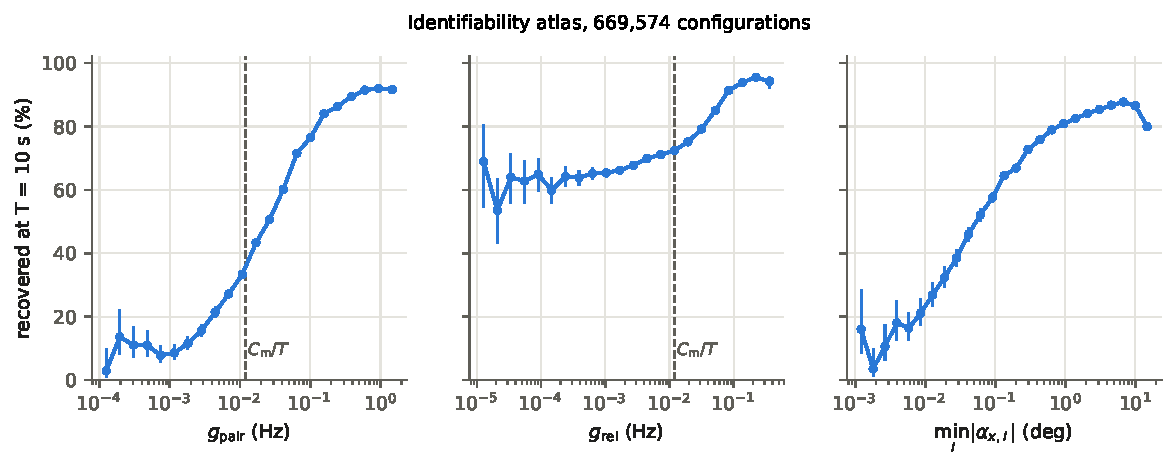
\includegraphics[width=\textwidth]{figures/E1_atlas.pdf}
\caption{The identifiability atlas: recovery probability at $T{=}10$\,s
against the three margin coordinates (Wilson 95\,\% bars, bins with
$\ge$20 configurations; 669{,}574 configurations). Dashed: the merge floor
$C_{\mathrm m}/T = 0.012$\,Hz. The derived detectability overlay
$\alpha_{\min}(T)$ is configuration-dependent and is not drawn.}
\label{fig:atlas}
\end{figure*}

\begin{table*}[t]
\caption{E2 (development scale): certified bounds on 121 fresh recovered
configurations (seed 20261008, $T{=}10$\,s), every parameter checked
against truth. The $10^{7}$-check campaign version of this table is still
pending; this run fixes the protocol and gives a first coverage figure.}
\label{tab:e2}
\centering\small
\begin{tabular}{lrrl}
\toprule
 & count & share & 95\,\%~CI\\
\midrule
configurations with all 18 bounds covering & 117/121 & 96.69\,\% & [91.81, 98.71]\\
median tightness (bound / true error), median over cases & \multicolumn{3}{l}{5.0}\\
\bottomrule
\end{tabular}
\end{table*}

\begin{figure}[t]
\centering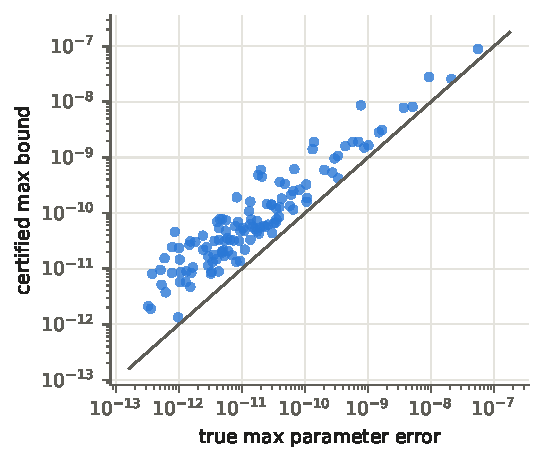
\includegraphics[width=0.75\columnwidth]{figures/E2_calibration.pdf}
\caption{Certified maximal bound against true maximal error, 121 fresh
recoveries (local development-scale run). Coverage = mass above the
identity line.}
\label{fig:cert}
\end{figure}

\begin{table*}[t]
\caption{E3, frequency-error law only. Population: the 18{,}402 configurations
unsolved at every rung, so the same cases appear at each $T$ (an
adaptive-campaign cohort, not the fixed-$T$ design; the pair-gap and
detectability laws still need the fixed-$T$ sweep).}
\label{tab:e3}
\centering\small
\begin{tabular}{lccl}
\toprule
law & derived & fitted (bootstrap 95\,\%) & note\\
\midrule
$\sigma(\hat N)\propto T^{\gamma}$ & $-3/2$ & $-1.58$ [$-1.59$, $-1.56$] &
$T{=}20$--$80$ only: $-1.42$\\
pair-gap inflation & $-2$ & pending & needs fixed-$T$ cohorts\\
detectability & $-1/2$ & pending & needs fixed-$T$ cohorts\\
\bottomrule
\end{tabular}
\end{table*}
\begin{figure}[t]
\centering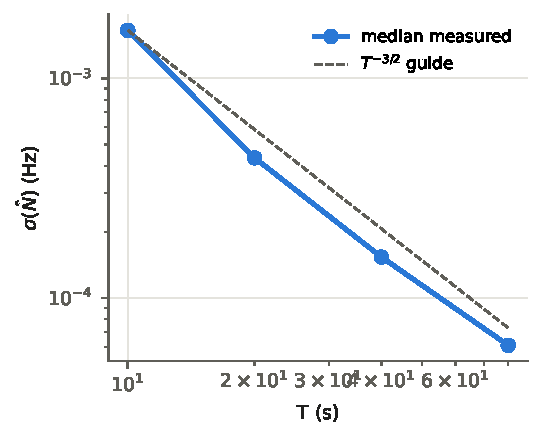
\includegraphics[width=0.75\columnwidth]{figures/E3_sigmaN.pdf}
\caption{Median certified $\sigma(\hat N)$ against $T$ for the always-unsolved
cohort, with the derived $T^{-3/2}$ guide.}
\label{fig:e3}
\end{figure}

\begin{table*}[t]
\caption{E4, ladder-censored version: 75{,}730 configurations failed at
$T{=}10$\,s with a numeric prescription and were later recovered on the
ladder. $T_{\min}$ is only known to lie in (previous rung, recovering rung];
the bisection design is still pending. Among the 9{,}902 configurations
unsolved at 80\,s with a numeric prescription, 9{,}594 (96.9\,\%) were prescribed
$T_{\mathrm{req}}>80$\,s, i.e.\ correctly predicted infeasible within the
ladder.}
\label{tab:e4}
\centering\small
\begin{tabular}{lr}
\toprule
recovered no later than the first rung $\ge T_{\mathrm{req}}$ & 91.48\,\% [91.28, 91.68]\\
$T_{\mathrm{req}}/T_{\mathrm{recovered}}$: p5 / p25 / p50 / p75 / p95 &
0.40 / 0.80 / 1.25 / 2.60 / 21.90\\
\bottomrule
\end{tabular}
\end{table*}
\begin{figure}[t]
\centering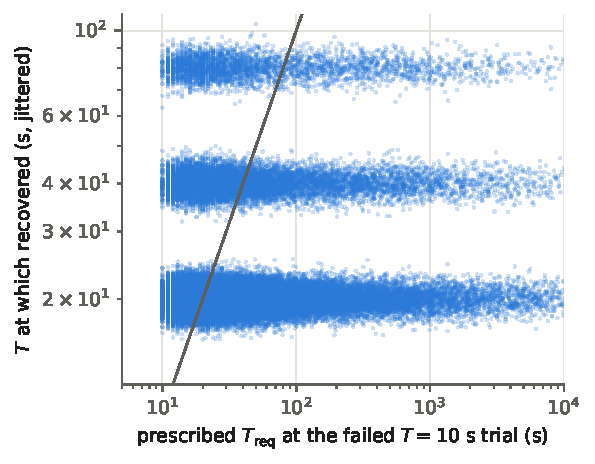
\includegraphics[width=0.75\columnwidth]{figures/E4_prescription.pdf}
\caption{Prescribed $T_{\mathrm{req}}$ against the rung that recovered the
configuration (vertical jitter for visibility); identity line drawn.}
\label{fig:e4}
\end{figure}
